\documentclass{report}


\usepackage[utf8]{inputenc}
\usepackage[T1]{fontenc}
\usepackage[francais]{babel}
\usepackage{lmodern}
\usepackage{titlesec}
\usepackage{graphicx}
\usepackage{xcolor}
\usepackage{caption}
\usepackage[pdfborder=0]{hyperref}
\usepackage{textcomp}
\usepackage{amsmath}
\usepackage[top=3cm, right=3cm, bottom=3cm, left=3cm]{geometry}
\usepackage{array,multirow,makecell}
\usepackage{listings}
\setcounter{secnumdepth}{3}
\setcounter{tocdepth}{3}
\setcellgapes{4pt}
\makegapedcells
\newcolumntype{R}[1]{>{\raggedleft\arraybackslash }b{#1}}
\newcolumntype{L}[1]{>{\raggedright\arraybackslash }b{#1}}
\newcolumntype{C}[1]{>{\centering\arraybackslash }b{#1}}


%pas necessaire ce qui suit
\usepackage[pages=some]{background}
\backgroundsetup{
	scale=1,
	color=black,
	opacity=0.1,
	angle=0,
	contents={%
		
\includegraphics[width=\paperwidth,height=\paperheight]{ulbback.jpg}
	}%
}


\title{Résumé de cours \\
	\vspace{10pt} \begin{Huge} \begin{bf} \og Les fondements de l'informatique \fg \end{bf} \end{Huge} \\
	INFO-H200 }

	 

\date{\vspace{100pt}  2015 }

\author{Raphael HANNAERT }

\titleformat{\chapter}[hang]{\bf\huge}{\thechapter}{2pc}{}

\begin{document}



\maketitle

\tableofcontents
\newpage

\chapter{Codage et traitement de l'information : le binaire}

\section{Fonctionnement global d'un ordinateur}

Le fonctionnement de l'ordinateur peut globalement être séparé en trois parties.
Les entrées, ou informations, sont d'abord {\bf stockées} puis {\bf traitées} et enfin {\bf transmises} (-> sorties).
La partie de traitement est celle la plus intéressante car la plus cognitive. En effet c'est celle qui nécessite des {\bf programmes}. Le traitement qui consiste en calculs,comparaisons,recompositions des informations est le fait du processeur et de ses deux unités : l'unit de commande (CU, control unit) qui séquence et choisit les opérations à effectuer et l'unité arithmétique et logique (ALU, arithmetic and logical unit) qui les effectue.

\section{Alan Turing et la prémière machine virtuelle}
C'est à Alan Turing qu'on doit la première machine universelle, spectaculaire dans sa conception, qui aurait permis de déjouer des navires Allemands lors de la guerre 40-45 grâce aux facultés de décryptage que celle-ci présentait.
Elle pouvait éxecuter n'importe quel programme en prenant une succesion d' {\bf états }. La machine peut lire ou écrire sur un très long ruban composé d'une suite de cellules qui fait office d'organes entrées-sorties mais aussi de mémoire puisqu'il peut mémoriser les écritures produites lors d'itérations précédentes. Chaque fois qu'il en reçoit l'ordre, le ruban est déplacé vers la gauche ou vers la droite par pas de longueur fixe, alternant simplement la celulle présentée au dispositif de lecture-écriture. En fait la machine peut prendre différents états internes si bien qu'elle peut présenter différents comportements pour de mêmes entrées en fonction de l'état dans lequel elle se trouve. Ainsi elle peut fonctionner par exécution d'une suite d'instructions(programme) sous la forme "Si la machine est dans l'état m et que la cellule lue contient le symbole + ou rien, alors la machine remplace ou non ce symbole, déplace le ruban vers la gauche ou vers la droite, et adopte le nouvel état n". C'est pour cela qu'on dit que la machine est {\bf universelle}, car elle peut effectuer toutes les tâches voulues en fonction du programme rentré. Schéma et exemple concret dans le livre pages 14-15.

\section{Le binaire : en stockage et en traitement}

Encore présent dans nos machines actuelles, le {\bf binaire} présente de nombreux avantages : \\
-La perception binaire est {\bf facile} à concrétiser et est plus économique, seulement deux états étant possibles: soit le courant passe, soit il ne passe pas. \\
-C'est plus {\bf robuste} et résiste bien mieux aux perturbations. Une fonction ne serait pas genée par du bruit vu que uniquement les deux états sont possibles et pas ceux intermédiaires (CF schéma prise de notes).\\
-Le circuit électronique binaire peut-être étroitement relié à la logique Booléenne, en effet l'équivalent électronique de AND et OR serait qu'un certain type d'assemblage entre circuits doit permettre, dans un premier cas, que deux circuits faisant ciruler un courant en entrée le fassent circuler en sortie et, dans le deuxième cas, qu'il suffit que l'un des deux soit alimenté pour que le courant appraraisse en sortie.\\
-Le binaire permet de stocker des donnés de manière permanente (magnétisme, optique, électronique,...).\\

En conclusion toute information est stockée et traitée en binaire.

\section{Le Transistor (transfer resistor)}
La première vague des ordinateurs a été lancée grâce aux développements de constituants importants tels que les bandes magnétiques, le disque magnétique(bouleversement dans le stockage et le traitement de l'information) et surtout le transistor qui feront leur apparition dans les ordinateurs dans le milieu des années soixante et dont le fonctionnement repose sur des phénomènes électroniques complexes.

Il s'agit d'un composant informatique composé notamment de silicium (semi-conducteur) à doper ou non avec du phosphore ou du bore et selon la combinaison, qui amplifie ,bloque ou inverse le courant suivant les conditions auxquelles le transistor est soumis, servant ainsi d'interrupteur qui réalise ces opérations à une vitesse extrèmement rapide. Il a remplacé l'ancienne technologie en place à savoir {\bf les tubes électronique}.


\begin{center}
	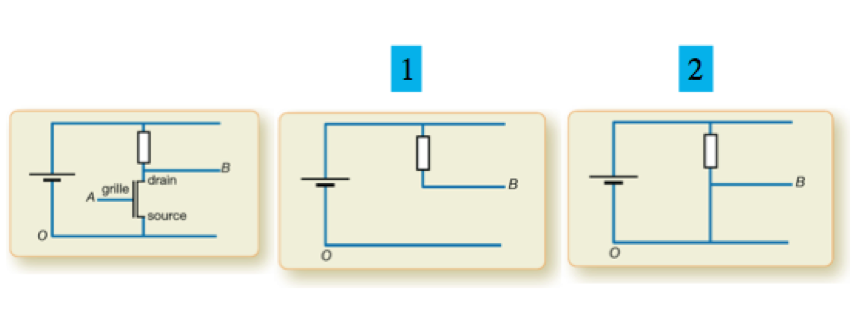
\includegraphics[ scale=0.4]{Transistor0}
\end{center}


Typiquement un processeur moderne contient des centaines de millions de transistors qui sont gravés ensemble pour ne pas devoir les assembler comme dans le temps,requérant une extrême précision.\\\\

Augmenter considérablement le nombre de transistors permet d'augmenter la capacité de traitement et de réduire le délai de transmission entre deux transistors mais augmente aussi les quantité de chaleur dégagée, la complexité et le coût ainsi que la possibilité d'avoir des effets quantiques tels que l'effet tunnel, provoquant des dysfonctionnements.

Globalement, comme prévu par la loi de Moore, la densité des transistors sur une puce double tous les 18 mois.

Plusieurs alternatives aux transistors sont en tentative de dèveloppement, notamment les nanotubes de carbone qui sont très résistants et capables de différentes propriétés électroniques et qui peuvent améliorer considérablement les perfomances des processeurs grâce aux diminutions des temps d'accès mémoire. En effet le basculement  (passage 0 $\leftrightarrow$ 1) par l'application d'une force électrostatique peut s'effectuer à des vitesses cent fois plus grandes que les bistables. Cependant les nanotubes se déteriorent lorsqu'ils sont mis en contact...\\
Une autre technologie prometteuse est l'utilisation de la lumière pour les opérations binaires car sa vitesse est imbattable.

Selon la disposition des transistors ( série, parallèle), on peut réaliser les différents fonctions booléennes ( and, or , nor, xor,...), on comprend donc mieux pourquoi nous avons dit plus haut qu'un circuit électronique s'apparentait à un circuit logique.

\begin{center}
	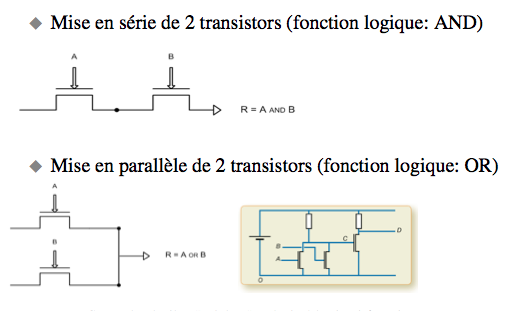
\includegraphics[ scale=0.6]{transist0}
\end{center}

NB : Que ce soit pour le AND ou le OR, si A = B = 0 le résultat logique sera 0. Si A = B = 1 le résultat vaudra 1.\\

Le schéma suivant illustre la représentation schématique de la logique binaire.


\begin{center}
	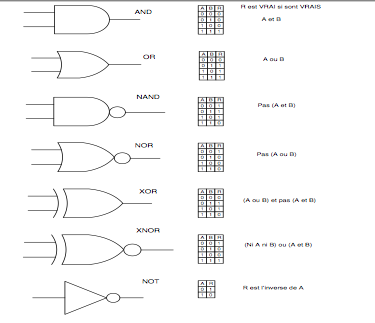
\includegraphics[ scale=0.8]{trans0}
\end{center}



Au niveau de la mémoire on a des éléments à deux états stables, d'où leurs noms : les bistables (flip-flop). Grâce à un circuit bistable on peut mémoriser un bit.

Le schéma ci-dessous montre un bistable formé de 2 NOR associés en boucle. En effet la sortie du premier est l'entrée de l'autre et inversement. La valeur peut donc être piègée à un moment donné et restera stable tans que rien ne se produit en S et R. Le bit sera donc stocker sous forme de 0 ou 1 c'est à dire que sa valeur sera mémorisée, c'est la base de la mémoire électronique (RAM) sur laquelle nous reviendrons plus loin.
Nommons la sortie de Na P et celle de Nb Q et supposons qu'on veuille mémorisée la valeur 1 grâce à Q. Pour cela on rentre en S la valeur 1 et pour toute valeur actuelle de Q P vaudra 0 ( car NOR) et comme R est à 0 ( sinon pas de sens car revient à vouloir écrire 0 et 1 au même endroit) et donc Q passe à 1 et est mémorisé tant qu'on ne modifie pas les valeurs en R et S car le circuit forme une boucle infinie.
 Ainsi en combinant des bistables on peut mémoriser plusieurs bits, et en faire des registres qui permettent leur lecture. Chaque niveau de complexité est accompagné d'un nouveau niveau d'abstraction. Cette démarche vers l'abstraction est une des caractéristiques de l'informatique, sa nature "fractale". Tout ordinateur peut être construit par la réplication d'un seul type de porte électronique, en de multiples exemplaires connectés d'une manière extrêmement élaborée.
\begin{center}
	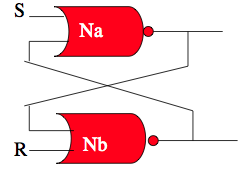
\includegraphics[ scale=0.6]{memoire0}
\end{center}



Sur le 1 er schéma ci-dessous on observe les deux états stables de A et B qui satisfont au circuit. En effet les "non" sont les équivalents des NOT du tableau vu précédemment qui correspondent à "A est l'inverse de B"
et présentant donc la stabilité si ceux-ci sont effectivement différents ( 0 et 1 ou 1 et 0 respectivement).


\begin{center}
	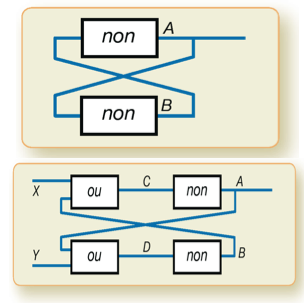
\includegraphics[ scale=0.6]{memoirebit0}
\end{center}
DEUXIEME SCHEMA A VERIFIER 

Le 2ème schéma montre comment on peut mémoriser une valeur entre 0 ou 1 et, en activant une entrée (X ou Y ici), comment change la valeur mémorisée.
En effet, si A = 1 les deux portes "ou" sont neutres. Mais si l'entrée X = 1, comme le "OU" ne permet pas d'avoir simultanément A et X qui valent 1, focément A prend la valeur 0. A nouveau, si on fait passer le Y à 1 par le meme raisonnement A prend... \\
Ainsi on peut développer des mémoires plus importantes en combinant des bistables pour former des registres de bistables.
Par exemple un registre à 4 bistables constituera une mémoire de 4 bits.\\

Le transistor peut également effectuer des opérations arithmétiques, en combinant un XOR qui additione les bits ( 0 + 1 donne 1, 0 + 0 donne 0 et 1 + 1 donne 0 ) avec un AND qui retient ( c'est à dire vaudra 0 si 0 et 0 ou 0 et 1 et vaudra 1 si 1 et 1, ce qui suit bien le principe du AND, revoir la liste des expressions en logique binaire plus haut si un doute subsiste). 


\begin{center}
	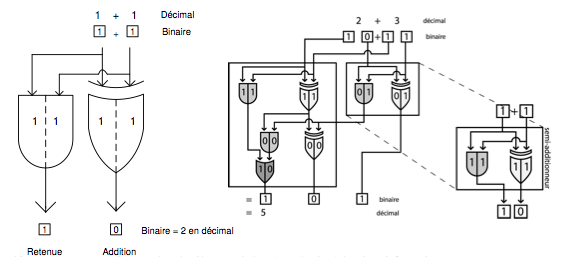
\includegraphics[ scale=0.6]{transisto0}
\end{center}

NB: On notera sur le schéma de droite les différentes combinaisons de retenues et additions pour sommer 2 + 3.
L'additionneur est construit avec autant d'étges qu'il y a de rangs de bits à additionner. Chaque étage est consituté par un demi-additionneur réalisée avec une porte XOR pour réaliser l'addition et d'une porte AND pour s'occuper de la retenue. La retenue du rang n est combinée avec l'addition du rang n+1 pour produire le résultat de l'addition du rang n+1. Le report du dernier étage est pour sa part ignoré. 

Finalement, on retiendra que les transistors en série réamplifient le signal qu'il reçoivent, que la modification du potentiel d'entrée change le potentiel de sortie avec un temps de changement de l'ordre de la nanoseconde mais justifiant donc le délai de réponse, et que les transistors permettent d'effectuer des calculs en plus de raisonner et mémoriser.

\section{Traitement de l'information : le binaire}

\subsection{Introduction au binaire}

Le sens(valeur) d'un {\bf bit} dépend de son contexte d'utilisation, il est donc nécessaire d'établir des standards, par exemple pour le codage des caractères informatiques.
Initialement il y avait {\bf ASCII}, mais ne présentait que 7 ou 8 bits, soit 128 ou 256 espaces de stockage d'un caractère (posant un problème pour des langages tels que le chinois...) donc 256 possibilités ( $\rightarrow$ pour les nombres on peut stocker de 0 à 255).

Ce qui n'était pas suffisament donc {\bf UNICODE} a été développé, constitué de 16 ou 32 bits ($2^{16}$ ou $2^{32}$ caractères différents possibles à stocker). Ce qui prend pas mal de place.

Finalement {\bf UTF-8} , une déclinaison de UNICODE qui est plus ingénieuse. Elle permet de coder les caractères les plus fréquents sur le - de bits $\rightarrow$ Codage du caractère en fonction de sa fréquence d'utilisation. Cette réduction du nombre de bits en fonction de la fréquence des caractères usités est propre au mécanisme de compression d'information que nous allons découvrir par la suite.




Soit des chiffres entiers non signés codés sur 8 bits (  = 1 octet $\simeq $ 1 byte)\\
NB: J'ai mis le signe $\simeq$ car en anglais comme en français, si l'on veut explicitement désigner une quantité de huit bits, on utilise le mot octet ; tandis que si l'on veut exprimer l'unité d'adressage indépendamment du nombre de bits, on utilise le mot byte, qui maintenant vaut 8 bits dans notre domaine d'étude mais dans d'autres domaines ou précedemment il a pris d'autres valeurs (5,6,7,9).\\

\begin{center}
	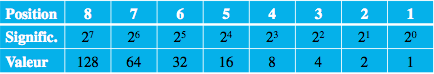
\includegraphics[ scale=0.6]{binaire0}
\end{center}

La clé permet d'interpréter les bits. \\\\
Par exemple 01010101 donnera :
\begin{center}


 0 x 128
+ 1 x 64 
+ 0 x 32
+ 1 x 16
+ 0 x 8
+ 1 x 4
+ 0 x 2
+ 1 x 1

= 85
\end{center}

Et de la même façon 11111111 = 255, puisque 00000000 = 0.\\

Le schéma ci-dessous permet de trouver la représentation binaire de tout nombre. Il est nécessaire d'être familier avec cette conversion !
L'exemple convertit 11 en 1011.

\begin{center}
	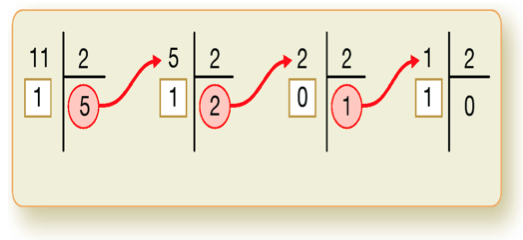
\includegraphics[ scale=0.6]{binair0}
\end{center}

On conclura que les entiers non-signés codés sur x bits permettent de stocker les valeurs allant de 0 à $2^{x}-1$

\begin{center}
	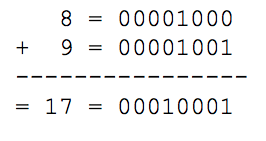
\includegraphics[ scale=0.6]{add0}
\end{center}

\subsection{Nombres entiers négatifs  } 

Maintenant si on désire représenter un signe négatif, il est donc nécessaire de dédier 1 bit au signe.
La notation dite en {\bf 2 complément} permet de coder aisément les nombres binaires en prenant la notation binaire de la valeur absolue du nombre, en y inversant chaque bit et en ajoutant 1 ( en binaire ) au résultat.
Ce qui donne pour coder 3 sur 4 bits : 0011 $\rightarrow $ -3 = 1100 + 0001 = 1101 \\
NB: on remarquera que le 1er bit, "le bit le plus significatif", nous informe sur le signe. Ainsi on peut stocker sur x bits les valeurs de $-2^{x-1}$ à $2^{x-1} - 1$. Cette notation permet de n'avoir qu'un seul zéro et de pouvoir traiter l'addition de nombres négatifs et positifs de la même manière. Le bit le plus significatif ou MSB(most significant bit) sera à 0 pour les nombres positifs et à 1 pour les négatifs.

\begin{center}
	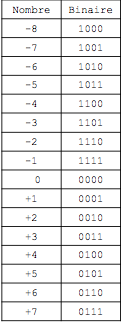
\includegraphics[ scale=0.6]{bin0}
\end{center}

Un peu d'arithmétique élémentaire en 2'complément: \\
\begin{center}
EX1\\ 0011 (3) \\
+ 0010 (2)\\
= 0101 \\
EX2\\0011 (3)\\
+ 1110 (-2)\\
= 0001 (1)  \\(on s'est débarassé du bit en trop)\\
EX3\\ 1010 (-6)\\
+ 1100 (-4)\\
= 0110 $\rightarrow$ OVERFLOW \\(détectée par le fait que le bit significatif de la somme (0) est $\neq$ de ceux des deux nombres (1), l'addition est donc infaisable d'où le Overflow.

En quelque sorte la notion de différence disparait, on somme juste des termes signés. ( 4 + (-3)).
Il y a Overflow quand le nombre ne tient pas sur le nombre maximum de bits dont on dispose.\\


Par le procédé ADD and SHIFT on ramène une multiplication à une addition.
\begin{center}
	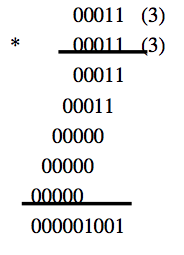
\includegraphics[ scale=0.6]{mult0}
\end{center}

\end{center}

\subsection{Nombres à virgule flottante}

Un nombre réel est constitué de 3 composantes à savoir son {\bf signe}, son {\bf exposant} et sa {\bf mantisse} ( partie après la virgule). 64 sont répartis de la manière suivante : 1 bit pour le signe, 11 pour l'exposant et 52 pour la mantisse.
L'exposant est compris entre -1022 et 1023, on le trouve en soustrayant 1023 ( CF plus bas).


\begin{center}
	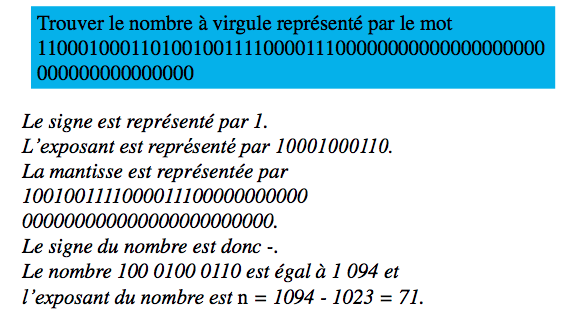
\includegraphics[ scale=0.4]{flo0}
\end{center}




\begin{center}
	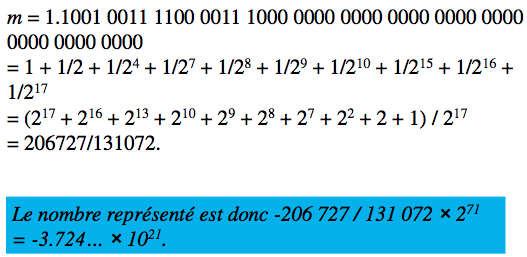
\includegraphics[ scale=0.4]{floa0}
\end{center}

Actuellement il existe des ANSI/IEEE standars pour ces représentations et opérations des virgules flottantes. Tous les processeurs les traient de la même façon.

Les additions et soustractions sont plus compliquées que les multiplications car il faut aligner les nombres (SHIFT) puis renormaliser le résultat. Pour la multiplication, il suffit de faire un shift final.

Il y a un grand nombre d'opérations arithmétiques qui portent et sur l'exposant et sur la mantisse.\\

\section{Images et sons}

Si on vise l'économie, ce qui en matièe de stockage est assez courant, certaines images peuvent être codées juste à partir des propriétés géométriques des différents éléments qui la composent. Par exemple un cercle dans une image est défini par les coordonnées de son centre au sein de l'image, par son rayon et par sa couleur. En général l'image est perçue comme un ensemble de segments paramétrés positionnés relativement l'un à l'autre. C'est la version {\bf PostScript} : On utilise un codage dit "vectoriel", permettant de limiter l'espace. L'avantage est que chaque élément peut être facilement redimensionné.\\En revanche il n'est généralement pas possible de recoder osus forme vectorielle une image acquise, par exemple, au moyen d'un scanner ou d'un appareil photo. Dans la version {\bf BitMap}, on code une image à partir de la superposition sur celle-ci d'un quadrillage avec un contenu plus ou moins fin. \\
Encore utilisée actuellement, cette version découpe l'image en Pixels ( Picture Element Image) et stocke octet par octet. Pour stocker un pixel coloré il faut généralement 3 octets ( 3 x 8 bits) pour les 3 couleurs primaires. La fidélité de la représentation est fonction de la densité du quadrillage(on parle de résolution de l'image) et de la richesse des nuances dans la description de chaque cellule.\\








Le son est un phénomène physique ondulatoire. Cette représentation simple est fidèle à la réalité mais elle implique une succession continue de valeurs,elles-mêmes continues, alors que l'ordinateur n'accepte de stocker et de traiter l'information que si celle-ci lui est présentée sous forme binaire. Il est donc indispensable de convertir les signaux continus en valeurs numériques entières et puis en binaire. On opère donc à une {\bf discrétisation ou digitalisation ou enore numérisation}.
L'onde est échantillonnée dans le temps et chaque échantillon est codé sur un certain nombre de bits. C'est le rôle de L'Analog to Digital Converter (ADC). La précision dépend de la fréquence d'échantillonnage et des intervalles de numérisation (qui doivent être respectivement la plus grande et les plus petits possibles) pour se rapprocher du signal d'origine.

\begin{center}
	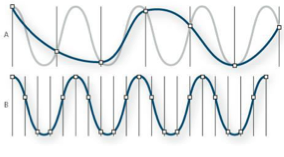
\includegraphics[ scale=0.6]{s0}
\end{center}

Ensuite pour rejouer le son il faut le reconvertir, cette fois-ci l'opération est effectuée par le Digital to Analog Converter (DAC).\\
Par exemple en téléphonie commutée, la voix est généralement transmise sous forme analogique jusqu'au commutateur où elle est échantillonnée 8000 fois par seconde et codée sur 8 bit. La voix est dès lors transmise avec un débit de 64 000 bits par seconde.\\

Dans le son comme pour les images, c'est la sensibilité de l'oeil humain qui détermine la richesse de la palette de couleurs perceptibles et donc par déduction le nombre de bits nécessaires pour permettre toutes les nuances possibles.\\

\section{Regroupement et compression des données}

Sans les mécanismes de compression, il faudrait près de 86Go pour une heure de film. On atteint ici des volumes d'information qui dépassent largement la capacité de stockage des supports. Il est donc indispensable de compresser les images et autres au maximum par des technologies suffisament standardisées pour que les dispositifs logiciels de visualisation s'y retrouvent.\\
Rappel : Byte $\neq$ Bit, le byte étant généralement plutôt une mesure de stockage et le bit de vitesse de transmission.\\ Par ailleurs, pour anticiper sur la suite dont les supports magnétiques et optiques, on peut déjà préciser que les bits y sont groupés en bloc de plus grande taille ( ce qui permet de tout déposer et extraire en un coup) par exemple en "secteurs" ( 52 octets.\\
La notation hexadécimale est une écriture plus concise que le binaire, c'est une manière simple de représenter un demi-octet à l'aide des chiffres de 0 à 9 et des lettres majuscules de A à F.
Regroupement de l'information : \\
	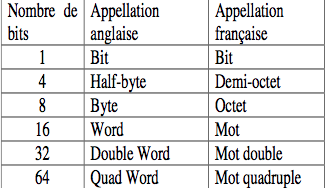
\includegraphics[ scale=0.4]{tableau0}
	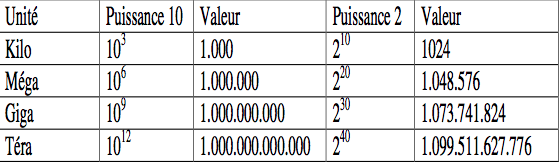
\includegraphics[ scale=0.4]{table0}

La réduction du poids des données peut se faire suivant deux approches :\\

\subsection{Compression de l'information(Zip,Jpeg,MP3,...)} 
Un mécanisme de compression des données est un processus totalement {\bf réversible} et le seul qui soit acceptable pour des informations textuelles ou numériques pour lesquelles aucune perte n'est à l'évidence tolérée.Le fait de coder les caractères les plus fréquents sur moins de bits est un exemple typique de compression. Ce processus exploite les mécanismes de redondances : une lettre ou un mot ou encore un pixels qui revient souvent sera codé sur moins de bits. Si on connait tables de traduction on peut dézipper et donc lire l'information qui a été codée de manière à prendre - de place, cette table est indispensable !

\subsection{ Compaction de l'information}

C'est une approche alternative qui concerne davantage les sons et les images. Le compactage consiste à alléger le codage des données tout en consentant une dépréciation de la qualité de l'information, considérée comme acceptable.
Ce mécanisme perd de l'information, l'information est donc quelque peu dégradée. (suppression de fréquences inaudibles, diminution de la résolution d'une image,...) C'est un processus {\bf irréversible}, l'information dégradée ne peut être reconstituée dans son état original. Cependant le gain en volume de stockage est souvent aussi considérable qu'irréversible.\\
La compression est symétrique, pas la compaction. La notion de symétrie sera expliquée dans la partie encryptage de l'information.\\


Il est intéressant de noter que les films sont assez facilement compressés car on ne stocke pas les images mais les {\bf différences} entre les images qui composent le film. ( Car les images sont souvent répétitives à peu de choses près).\\

\subsection{Corriger l'information}

Quel que soit le mode de regroupement choisi, ce dernier a toujours pour objectif de constituer des ensembles de bits afin d'en discrétiser le transfert. Quand on transfère de l'information il est nécessaire de le faire par nombre prédéterminés de bits, de taille fixe. Comment remarquer une erreur de transfert par exemple un bit 0 converti en 1 lors du transfert d'un octet ? Une première solution serait de joindre à l'octet deux copies, puis de regarder dans les suites de triplés là où justement on a pas un triplé, c'est là que le bit a changé de valeur, l'erreur est repérée mais ce fut onéreux en bits. Une autre méthode plus économe est celle du bit dit {\bf "de parité"}. Ce bit est mis à 1 si le nombre de 1 dans l'octet est pair et à 0 sinon. Cela permet de repérer une erreur de transfert pour un nombre impair de bits en erreur. 
Corriger des erreurs recquiert l'{\bf insertion de bits supplémentaires} (redondants)\\

\subsection{Encrypter l'information}
L'encryptage des données consiste en la protection de celles-ci. Toute technologie de cryptage se base sur la connaissance d'une clé qui détient toujours le secret de l'écriture et de la lecture et qui est unique si on parle de cryptographie {\bf symétrique}.Cette seule clef doit donc parvenir au destinataire le plus discrètement possible,ce qui est complexe,si bien que dans un processus de communication on préfèrera recourir à une cryptographie {\bf asymétrique}. Celui-ci fonctionne sur le principe de clef publique - clef privée : le destinataire reçoit la clef publique et encrypte le message que seul vous, avec la clef privée pouvez décrypter.
Donc l'algorithme qui permet de transformer l'information est connu de tous mais pas la clef.


\chapter{Fonctionnement intime du processeur}

\section{Von Neumann et les éléments du processeur}

Von Neumann a défini l'architecture d'un ordinateur en décrivant les caractéristiques de ses cinq composants essentiels :\\
-{\bf L'unité de commande} qui contrôle le déroulement successif des instructions du programme.\\
-{\bf L'unité arithmétique et logique} qui effectue les opérations de calcul et de comparaison.\\
-{\bf La mémoire centrale } qui contient les programmes et les données.\\
-{\bf L'unité d'entrée} qui s'occupe de l'acquisition des données.\\
-{\bf L'unité de sortie} qui gère la restitution des résultats.\\

L'unité de commande(CU,control unit) et l'unité arithmétique(ALU,arithmetic and logical unit) forment deux entités distinctes, la première s'occupant de ce qu'il faut faire et la deuxième le réalisant. Les deux sont généralement regroupées sous l'appelation {\bf "unité centrale de traitement" (CPU, central processing unit) ou "processeur"}\\

\section{PHO}
Un ordinateur exécute des programmes, c'est-à-dire une séquence d'instructions. Une fois traduites en instructions élémentaires, le PHO (Petit Homme Ordinateur) prend le relais.\\
Ce PHO a été conçu par Von Neumann.\\
Concrètement, le PHO cherche l'adresse de l'instruction, il la lit et la décode avant de l'exécuter et finalement, il incrémente le compteur.\\
C'est ce qu'on appelle l'Informatique Séquentielle et Programme chargé et stocké en mémoire, impliquant un CPU, ALU des mémoires et registres.\\  Les {\bf registres} sont des dispositifs auxiliaires associés au processeur et capables, pendant un temps limité, de mémoriser ou de transformer les informations. Les registres se distinguent de la mémoire centrale car ils ont une {\bf capacité de stockage extrêmement réduite}. Ils sont en petit nombre et isolés avec des emplacements et fonctions spécifiques, alors que la mémoire centrale est constituée d'un très grand nombre de cellules adjacentes, différenciées par leur seule adresse. \\ 


\begin{center}
	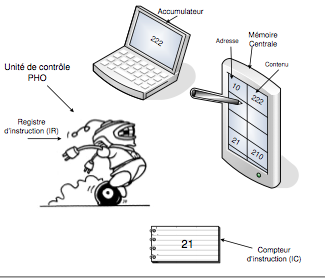
\includegraphics[ scale=0.6]{PHO1}
\end{center}

Nous savons que chaque partie mémorisée est accessible par une adresse, c'est ce qui est représenté sur le schéma pour la {\bf mémoire centrale}, sachant que sur 64 bits on peut stocker $2^{64}$ infos en mémoire.
Le processeur contient trois registres.
Le {\bf registre d'instruction (IR)} stocke l'instruction. Pour la faire fonctionneur on nécessite {\bf l'accumulateur} et finalement le {\bf registre compteur d'instruction} est incrémenté pour que le programme puisse s'éxécuter.\\

Le PHO va donc chercher l'instruction à l'adresse 21 et y trouve l'instruction 21 et la met dans sa tête (registre d'instruction) Cette étape d'extraction de l'instruction est dénommée l'instruction "fetch".En fait ce n'est pas une extraction à proprement parler, mais une "copie" du contenu de la mémoire dans une autre zone mémoire ou un registre. 210 est séparé en 2 parties à savoir 2 et 10. Le 2 est la partie qui indique de quel type d'instruction il s'agit ( addition, transfert vers fichier A,...), c'est le {\bf code de l'instruction}. Par exemple si 2 représentait une addition : 10 serait ce qu'il faut additioner ou plutôt son addresse donc le PHO irait à l'adresse 10, y trouverait 222 comme valeur et l'additionnerait. A quoi ? A ce qu'on avait précédemment c'est à dire qu'il faut bien voir l'addition non comme A + B avec A et B deux valeurs données mais plutôt comme "je rajoute A" à ce que j'ai déjà dans {\bf l'accumulateur}. Donc la partie exécution se déroule et ensuite le IC est incrémenté de 1 et donc le PHO passe de l'addresse 21 à 22 pour une nouvelle instruction. En pratique 2 n'est pas une addition mais un déplacement de données comme dans 80\% des instructions.


\begin{center}
	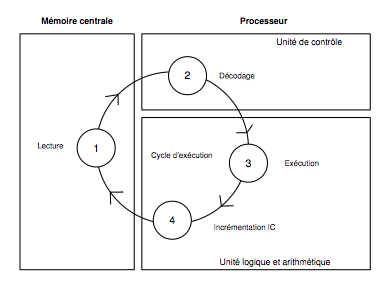
\includegraphics[ scale=0.6]{cycle1}
\end{center}
La partie décodage sépare 210 en 2 et 10.\\
C'est suivant ce schéma que TOUS les processeurs fonctionnent ! Cependant, ils diffèrent et sont incompatibles car chacun d'eux possède un ensemble d'instructions ou {\bf jeu d'instructions} qui lui est propre. Chaque processeur parle un langage particulier construit à partir de ses instructions élémentaires.
\\

Les quatre classes d'instructions élémentaires sont les {\bf déplacement et copie de données, les opérations Arithmétiques et Logiques, les opérations Conditionnelles et de Branchement ou sauts d'instruction (Conditionnels ou Inconditionnels), ainsi que les Opérations d'entrée/sortie avec les périphériques}\\
Les instructions sont composées de deux parties: {\bf le code instruction et l'adresse de l'opérande"}

Au début il n'y avait que des instructions élémentaires réalisées une par une mais ensuite on a développé des langages de programmation de haut niveau (LPH) dont une instruction réalise plusieurs instructions élémentaires.\\
Par exemple "c=a+b" est plus simple que la suite d'instructions élémentaires "load a,reg1","load b,reg2",... qui donnent le même résultat.\\

Les instructions qui suivent seront utilisées plus loin dans ce chapitre. Il est donc intéressant de lire leur signification. De même l'adresse des données et des instructions sera utile pour comprendre le 3ème tableau ( du LPH au binaire) mais n'est pas à retenir.

\begin{center}
	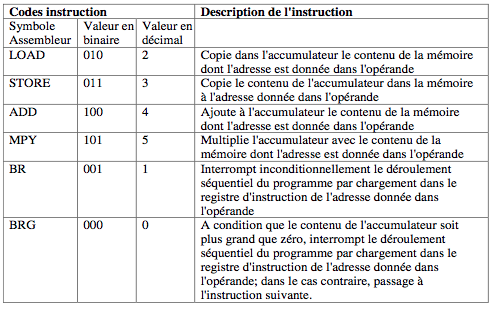
\includegraphics[ scale=0.6]{instruct1}
\end{center}


\begin{center}
	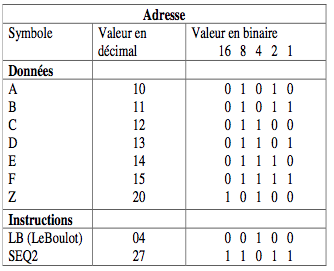
\includegraphics[ scale=0.6]{tab1}
\end{center}

Pour rappel l'ordinateur ne comprend que le binaire, il est donc nécessaire de traduire les données et les instructions en binaire pour qu'elles soient bien comprises.

\begin{center}
	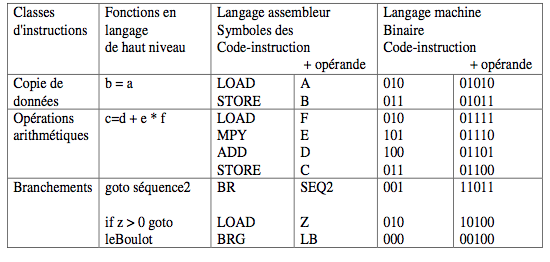
\includegraphics[ scale=0.6]{ta1}
\end{center}

On constate sur le tableau ci-dessus dans la deuxième ligne qu'il n'est pas nécessaire de Load E et D car les add et multiply le comprennent déjà et l'appliquent à l'accumulateur il n'est donc pas nécessaire de leur donner deux arguments.
Le store est nécessaire pour stocker la nouvelle valeur.

Les 3 tableaux ci-dessus constituent respectivement les actions "Copie de A vers B : b=a", "Opération arithmétique: c = d + e x f" et "Branchement et boucle: while z > 0 do LeBoulot".

Pour le branchement BRG, la rupture est conditionnée par la valeur de la donnée qui a été préalablement chargée depuis l'adresse 20 dans le registre accumulateur. Si le contenu du registre accumulateur, et donc la donnée Z, est $>$ à 0, le compteur d'instruction sera chargé avec l'adresse 5, le début de la séquence LeBoulot ayant pour symbole LB. Dans le cas contraire l'instruction suivante est exécutée. Pour le branchement BR qui termine la séquence LeBoulot, la rupture est inconditionnelle et on place dans le registre compteur d'instruction l'adresse 27 correspondant à SEQ2.\\
Les boucles sont un mecanisme essentiel de fonctionnement de l'ordinateur. 
\\Pour résumer, quelle que soit le processeur, une instruction début par un code instruction, constitué d'un certain nombre de bits qui après décodage, déclenchera une série de sous-opérations.Ce découpage en instructions élémentaires est fait par le {\bf séquenceur}.

\begin{center}
	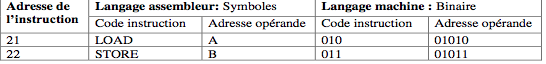
\includegraphics[ scale=0.6]{t11}
\end{center}

\begin{center}
	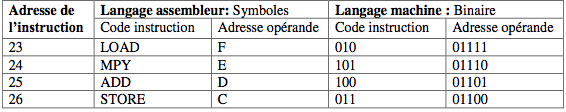
\includegraphics[ scale=0.6]{t21}
\end{center}

\begin{center}
	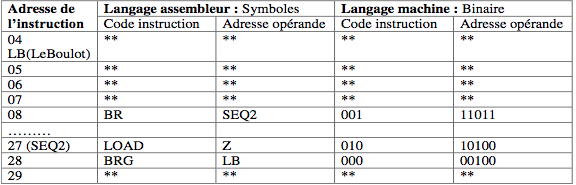
\includegraphics[ scale=0.6]{t31}
\end{center}


Toute l'informatique repose sur {\bf le principe de l'abstraction fonctionnelle}, en effet un ordinateur fonctionne à différents niveaux d'abstraction. On peut travailler à un niveau supérieur sans se soucier du niveau inférieur.

\begin{center}
electronique $\rightarrow$ logique $\rightarrow$  assembleur $\rightarrow$ langage de programmation
 \end{center}

Ainsi au fil des années on a augmenté dans les niveaux d'abstraction sans plus se préoccuper des niveaux en-dessous, ce qui permet au programmeur de prendre de la distance par rapport au processeur et de pratiquer une programmation plus proche de la manière de poser et de résoudre les problèmes.

\section{Eléments fondamentaux de l'architecture}

{\bf Les Registres}


Les registres ont déjà été définis plus haut.
Ils interviennent dans les instructions pour les données ou les adresses des opérantes et peuvent être chargés,sommés,permutés,translatés.
Le transfert entre registres conditionne la vitesse du CPU.\\

{\bf Les Mémoires}

Comme dit précédemment avec un MAR de 32 bits on peut aller jusque $2^{32}$ ( = 4 GigaBytes de mémoires principales) espace mémoire. Actuellement le MAR possède 64 bits.

LE MDR = 1 Byte et donc il faut accéder plusieurs bytes successivement, ou 2 ou 4 bytes. 



{\bf Les bus}

Ils peuvent êtres locaux et connecter des registres entre eux. Plus il y en a, plus d'information pourront êtres transmises simultanément, plus le CPU ira vite.

Ils peuvent également connecter le CPU à la mémoire et le CPU aux périphériques.

En général, les bus sont parallèles au sein du CPU et séries pour connecter des périphériques plus distants.

Un bus contient un ensemble de lignes avec données, adresses ou information de contrôle.

Ils seront approfondis plus tard.\\

\section{CISC vs RISC} 

Soit la problématique suivante : on dispose d'un processeur x32 (32 bits).
Ces 32 bits sont partagés entre le code et l'opérande et dont leur longueur et la place qu'ils occupent dépendent du nombre d'instructions.
Imaginons qu'il puisse éxecuter 256 exécutions ( 8 bits). Et supposons que si besoin de deux opérandes et que chacune tient sur 32 bits il faudra donc au total 8 + 2 x 32 bits soit 72 bits or on en dispose que de 32 ! ( car processeur x32). On dit qu'il y a {\bf problème d'adressage}.Cette problématique a donné naissance au débat entre les processeurs {\bf RISC et CISC}.\\

Les intructions d'un processeur {\bf CISC (Complex Instruction Set Computer) }seront de longueur variable, nombreuses et diverses, rendant plus complexes la lecture, le décodage et l'exécution des ces instructions par le processeur.

Dans un proccesseur {\bf RISC (Reduced Instruction Set Computer)}, les instructions sont de taille fixe et de format semblable (32 ou 64 bits pour la plupart des processeurs actuels)avec utilisation surtout de registres du processeur. Les instructions seront en nombre plus réduit et montreront une structure homogène,autorisant la conception de processeurs plus simples et généralement plus efficaces.\\

Intel a toujours favorisé le type CISC (pas Motorola qui sont les anciens processeurs des macs, maintenant aussi Intel). Mais il y a actuellement un retour des processeurs RISC dans les tablettes, smartphones, GPS. 
 


\begin{center}
	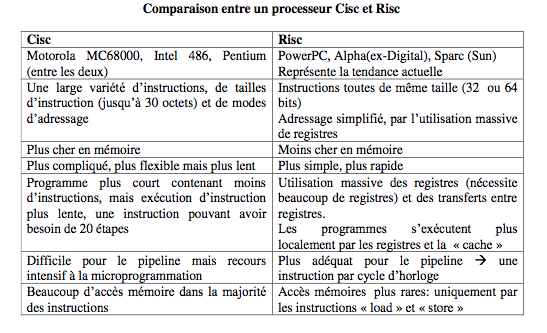
\includegraphics[ scale=0.6]{processeurs1}
\end{center}

La longueur de instructions, soit le nombre d'octets qu'elles nécessitent, est une préoccupation majeure lors de la conception d'un processeur. Qu'on soit en RISC où il est obligatoire de faire tenir chaque instructions dans la longueur canonique( 4 ou 8 octets) ou dans la version CISC où la longueur des octets est moins contraignante, il faut raccourcir ces instructions qui prennent de la place en mémoire,ce qui influe notamment sur le temps nécessair pour alimenter les instructions depuis la mémoire vers le processeur, sur leur temps d'exécution et donc sur la vitesse d'exécution des programmes. La limitation de la longueur des instructions ne peut se faire sur le code d'instruction, c'est pourquoi il faut limiter la taille des champs attribués aux adresses des opérandes surtout dans les processeurs RISC, vu le format unique de l'instruction. C'est pourquoi les porcesseurs de type RISC font un usage quasi exclusif pour leurs opérandes d'adressage par registre ou relatif (ces adressages sont expliqués dans la section suivante). Finalement, dans un processeur RISC, une addition s'effectuera à partir des données contenues dans les registres et préalablement recopiées de le mémoire centrale. En revanche, dans un processeur CISC, cette meme addition pourra s'effectuer directement à partir des données contenues dans la mémoire centrale.

On comprend maintenant pourquoi un programme dans sa version traduite en langage machine ou exécutable, ne peut s'exécuter que sur un type de processeur donné. Les processeurs parlent en effet des langages différents et ne se comprennent pas entre eux, bien qu'ils aient le meme mode opératoire.

\section{L'adressage}

On a vu qu'il y avait des différences fondamentales entre RISC et CISC, notamment que le RISC doit adresser beaucoup plus à partir des registres pour maintenir des adressages courts et donc des petites instructions.\\


Pour réduire l'espace pris par l'opérante on réduit la taille de l'adresse. On dit qu'il y a {\bf adressage}.\\ En fait, une partie de l'instruction étant déjà réservée pour le code d'instruction, il faut s'efforcer de réduire au maximum la taille des adresses. L'unique manière de limiter cette taille est de recourir à des modes d'adressages subtils permettant de réduire dans l'instruction le nombre d'adresses possibles et donc finalement le nombre de bits nécessaires à cet adressage. Une autre raison qui conduit à réduire la taille occupée par les adresses est le principe de localité, que nous retrouverons plus tard. En général, un programme, en s'éxécutant, n'utilise au fur et à mesure que des instructions et données restant proches dans la mémoire.



Il existe différents types d'adressage, dont certains peuvent se combiner.\\

\subsection{Adresse absolue} 
C'est l'adresse mémoire effective. nécessite 32 ou 64 bits, apportant dès lors un effet grossissant sur les instructions, effet croissant encore avec la multiplication des opérandes.\\
\subsection{Adresse registre}
Si on considère que certaines instructions ne porteront que sur des données contenues dans des registres, la taille de l'adresse peut se réduire considérablement au numéro du registre, comme il y a peu de registres. Ce mode d'adressage est très utilisé dans les processeurs RISC pour sa réduction ds tailles des instructions.\\
\subsection{Adresse relative}
l'adresse indiquée est un "offset" qu'on additione à une base chargée au préalable dans un registre afin d'obtenir l'adresse effective (adresse absolue). Une adresse relative est automatiquement de taille plus petite qu'une adresse absolue, de plus les données manipulées par un programme sont souvent de type matriciel ou vectoriel, toutes les données se suivant donc, ce qui rend l'usage de l'adressage relatif très utile.\\
\subsection{Adresse indirecte}
L'adresse renvoie soit vers une cellule de la mémoire centrale, soit vers un registre où se trouve l'adresse effective de l'opérande que l'on souhaite traiter. Ce mécanisme peut être répété. Ce principe sert plus à manipuler des adresses qu'à diminuer leur taille. Un exemple d'utilisation intéressante serait pour un programme qui doit effectuer une séries d'opérations sur une donnée dont on ignore l'adresse finale ou dont l'adresse peut varier au cours de l'exécution du programme. Peut être combiné avec l'adressage relatif pour faciliter la localisation et le traitement de données.\\ 
\subsection{Valeur immédiate}
Le champ opérande contient une valeur qui est utilisée immédiatement telle quelle, par exemple une valeur numérique.
Exemple : ADD Rn 5 qui se traduit par augmenter de 5\\
On voit sur le schéma ci-dessous l'illustration des différents types, tous aboutissant au même résultat : la valeur 123 est chargée dans l'accumulateur. Pour réduire l'espace utilisé par l'adressage des opérandes,il est indispenable d'éviter l'adressage absolu. En général il est préférable d'avoir un mécanisme de limitation de l'accès de la mémoire. C'est le principe de la mémoire protégée. Toute zone mémoire occupée par un programme est une propriéré privée et inaccessible par les autres programmes, sauf avec une pièce d'identification délivrée pat le système d'exploitation. Lorsque plusieurs programmes s'exécutent en même temps (multitâche), chaque programme se voit attribuer sa zone mémoire propre.
Finalement, on notera que le code de l'instruction aura également pour fonction d'informer le processeur sur le type d'adressage à utiliser.
\begin{center}
	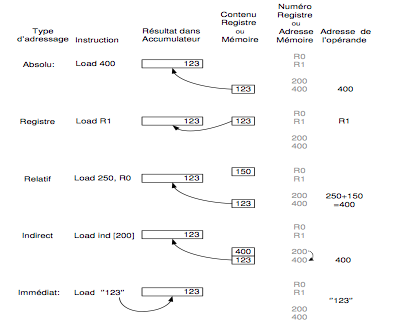
\includegraphics[ scale=0.6]{adressage1}
\end{center}

\section{Fonctionnement du processeur}

Tout le fonctionnement de l'ordinateur se ramène à des {\bf transferts de registres} et à chacun de ces registres correspond une utilisation spécifique. C'est cette vitesse de transfert que l'on caractérise avec les Ghz indiquant la vitesse du processeur. En effet le déroulement d'une instruction élémentaire correspond à plusieurs étapes atomiques. Donc si le processeur est qualifié de 1 GHz il pourra effectuer 1 Milliard de ces étapes atomiques par seconde.\\

Le {\bf séquenceur } est un peu le comme le poste central de commande qui aiguille les échanges entre registres, à l'image d'un chef d'orchestre. On l'approfondira dans la section suivante.

Le tableau ci-dessous reprend les principaux registres.

\begin{center}
	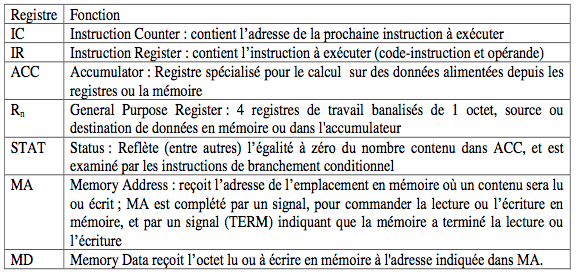
\includegraphics[ scale=0.6]{reg1}
\end{center}

On a déjà parlé du compteur d'instructions, le registre d'instruction et l'accumulateur mais rappelons brièvement leurs fonctions \\

\subsection{Compteur d'instructions CI}
Il contient {\bf l'adresse} de l'instruction à exécuter, et donc l'adresse mémoire d'où le processeur peut recopier cette instruction. Il est incrémenté pour passer à l'instruction suivante.
\subsection{Registre d'instructions RI}
Contient {\bf l'instruction} à exécuter, telle que le processeur l'a lue en mémoire à l'adresse donnée par le compteur d'instruction.Un fois l'instruction sotckée dans ce registre,c'est l'emplacement à partir duquel son décodage pourra etre entrepris par le séquenceur.
\subsection{Accumulateur ACC}
Effectue les opérations arithmétiques et logiques sur les données.
\subsection{Registre d'état STAT}
Donne l'état du proccesseur au terme de l'exécution de l'instruction. Par exemple il peut donner le résultat de l'accumulateur pour une instruction de branchement conditionnel qui teste le résultat d'une instruction précédente afin de décider quoi faire par la suite.
\subsection{Registres de travail}
Numérotés $R_0,...R_3$ sur le schéma, ils sont présents dans tous les processeurs mais en différents nombre, banalisés ou spécialisés. Ce sont eux qui différencient pour une large part les processeurs.

\subsection{Registre d'adresse et registre de données}
Par opposition avec les registres vus ci-dessus qui sont dits programmables car leur contenu est accessible au programme, le processeur contient d'autres registres intermédiaires qui ne sont pas directement visibles par le programme. Les registres d'adresse et de données gèrent les transferts entre le processeur et la mémoire centrale.\\
Le {\bf registre d'adresse RA} contient l'adresse du transfert mémoire et des commandes.\\
NB: Comme on a dit précédemment, pour la mémoire on ne fait pas de distinction entre une instruction et une donnée, elle ne le voit que comme des bits logés dans une adresse, à lire ou à écrire.\\
Le {\bf registre de données RD } contient soit la donnée à lire depuis la mémoire soit celle à écrire en mémoire.




\subsection{Important : Schéma de synthèse bloc du fonctionnement du processeur}




\begin{center}
	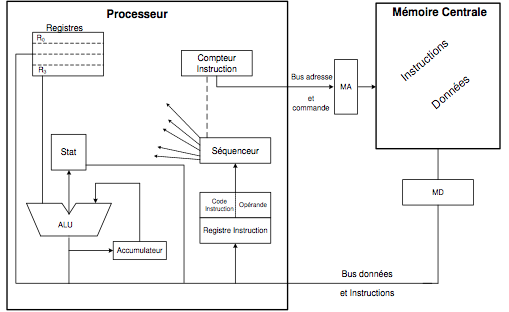
\includegraphics[ scale=1]{fond1}
\end{center}

\newpage

\section{Etapes primitives}
Le processeur exécute chaque instruciton en la découpant en étapes primitives ou étapes atomiques. La mise en oeuvre d'un organe du processeur revient à un transfert de registres, commandé par le séquenceur et consistant à copier dans un registre le contenu d'un autre registre ou à y écrire le résultat de la combinaison de plusieurs registres. Par soucis de stabilité il est important qu'il y ait un délai suffisant entre les différentes étapes, c'est pourquoi chaque étape doit se dérouler dans un temps prévu et défini par une cadence fixée par l'horloge interne du processeur. En fait le temps d'exéctuion d'une instruction est la somme des temps nécessaires à l'accomplissement de chacune des étapes. On verra dans la prochaine section comment accélérer le fonctionnement du processeur. Pour illustrer la découpe des instructions en étapes atomiques on va prendre l'exemple figurant sur la prochaine figure : la copie ou chragement LOAD du contenu d'un registre dans le registre accumulateur, suivie de l'addition ADD du contenu d'un autre registre. La première phase de l'instruction est {\bf la lecture} depuis la mémoire vers le processeur. En vue d'obtenir l'instruction à exécuter, son adresse en CI est copiée dans le registre RA, complétée par un ordre de lecture de la mémoire, CI est incrémenté de 1 pour contenir l'adresse de l'instruction suivante. Puis vient le deuxième cycle de base, où l'octet lu en mémoire est copié dans le registre d'instruction RI dès l'envoi par la mémoire du  signal TERM annonçant son arrivée dans le registre RD. On obtient donc le chronogramme logique de la figure correspondant à la lecture ou au chargement, qui nécessite deux cycles de base. La seconde phase est celle de {\bf l'exécution} qui est composée d'un seule étape, qu'on prenne le cas de LOAD ou ADD. Le chronogramme complet est donc en 3 étapes.

\begin{center}
	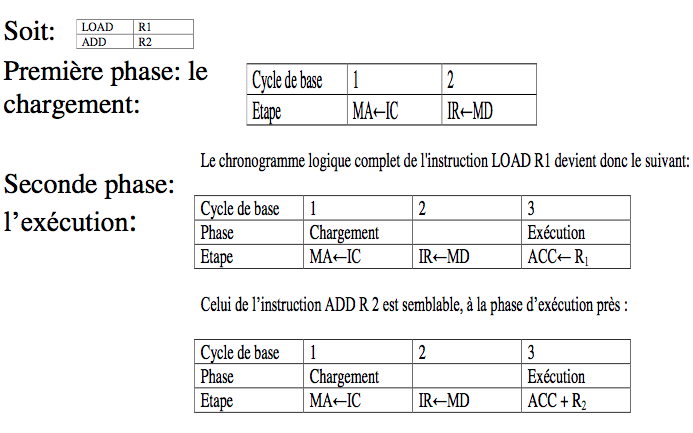
\includegraphics[ scale=0.4]{pipe2}
\end{center}

\section{Séquenceur}
Les transferts entre les registres s'effectuebt par des liaisons multiples parsemées de composants électroniques faisant office d'interrupteurs, de sorte que le signal électrique qui représente un bit n'y soit propagé qu'au bon moment, dans la bonne direction et vers le bon destinataire. Pour chaque type d'instructions, le séquenceur dispose d'une liste d'actions à réaliser selon une division spatiotemporelle. Comme dit plus haut le séquenceur est un peu le chef d'orchestre du processeur. Il existe des séquenceurs {\bf cablés} et des séquenceurs {\bf microprogrammés} Les premieurs recourent aux seuls circuits électroniques.Ce cablage devient rapidement complexe avec l'accroissement du nombre d'instructions et entraine des difficultés pour toute modification du processeur. On peut le résumer à rapidité, complexité et manque d'adaptabilité. Le séquenceur microprogrammé lui est un séquenceur programmable qui, pour chaque instruction à exécuter, va consulter une table avec les différentes étapes.

\section{Pipeline et parallélisme}
Le parallélisme est assez facile à comprendre.
On peut paralléliser les instructions élémentaires en multipliant le nombre de processeurs dans une même machine ou en améliorant le fonctionnement du processeur en utilisant le pipeline.
C'est le principe du temps vaincu par l'espace, où comme avec les autoroutes à plusieurs bandes, quand on vise à diminuer le trafic on étale.
En ramenant le séquentiel au {\bf parallélisme} on peut réduire la durée d'éxécution, c'est le {\bf pipeline}. Par opposition avec le déroulement des instructions élémentaires une par une, si ce ne sont pas les mêmes parties et transferts du processeurs qui sont concernés donc on peut superposer des instructions.\\


\begin{center}
	\includegraphics[ scale=1]{Pipeline2}
\end{center}

Il faut bien se rendre compte que ce parallélisme est rendu impossible si les instructions sont dépendantes les unes des autres. Par exemple on ne pourra pas effectuer en même temps les opérations c = a*b et f = c+d car la 2ème opération nécessite le résultat de la 1ère à savoir c.
De même une instruction conditionnelle dans une boucle sera conditionnée par la boucle précédente et ne pourra donc pas s'éxécuter en même temps.
On remarquera quand même que ces problèmes de dépendances entre instructions et d'instruction de branchement peuvent être résolus soit à la compilation, soit en créant des retards, soit en utilisant plusieurs pipelines ou encore en ré-ordonnant les instructions.
Une autre approche pour corriger ces problèmes liés aux branchements conditionnels est de dédoubler les unités de traitement du processeur. On traite dans deux branches séparées les deux possibilités de réponse à la condition. Une fois la réponse connue, les résultats de la séquence qui n'apas été choisie sont éliminés. Cela permet d'utiliser au mieux le pipeline.
 C'est le séquenceur qui dit que 2 instructions sont à exécuter en même temps. Certains processeurs actuels peuvent aller jusqu'à 40 étages de pipeline. Les processeurs RISC ont plus de facilité à recourir au mécanisme du pipeline vu la cimplicité et l'uniformité du codage d'instruction. Les processeurs CISC peuvent se rapprocher de ce type de fonctionnement en décomposant leurs instructions en une suite d'instructions adaptées au fonctionnement du pipeline.

Il existe un autre modèle de Pipeline, le {\bf superscalaire}, où les instructions sont séparées en fonction de sur quoi elles portent (Entier,virgule flottante et branchement) et chacun de ces types d'instructions est aiguillé vers un différent CPU. C'est un système multi-processeurs, actuellement Intel met jusque 8 processeurs sur une même puce
On notera finalement le cloud computing ou encore le grid computing qui consistent en des partage de tâches entre plusieurs ordinateurs et finalement le recours aux ordinateurs quantiques pour utiliser la superposition d'états en vue d'accélérer encore plus les processeurs mais encore rien de concret actuellement à ce niveau, juste des espérances...

\chapter{Les mémoires}




\section{Définitions et rappels}

\subsection{Classifications des mémoires}
Les mémoires sont les dispositifs qui permettent de stocker des informations, en quantité importante, et sans autre limite théorique que simplement matérielle. Vu leur petite capacité de stockage et leur spécialisation, les différents registres vus ne sont pas vraiment considérés comme des mémoire en ce sens. Les mémoires peuvent être classées en niveau selon leur capacité de stockage, leur niveau de résolution de leur adressage, leur temps d'accès et leur débit, ainsi que selon leur fiabilité, leur volatilité, leur encombrement physique ou leur coût.\\

\subsection{Mémoires vives, mémoires de masse et mémoire morte}
On peut faire une première distinction suivant la nature technique de la mémoire : Il y a d'une part les mémoires qui se remplissent et s'animent au cours de l'exécution des progammes mais dont le contenu s'efface sitôt que l'ordinateur est mis hors-tension, les mémoires {\bf vives}, et d'autres part les mémoires permanentes dont le contenu est préservé entre deux utilisations des programmes ou de la machine, les mémoires de {\bf masse}. Les mémoires vives s'occupent d'alimenter le processeur en instructions et en données, et les mémoires de masse assurent la permanence des données au-delà de l'exécution ponctuelle d'un programme.  Un troisième type de mémoire existe, dont l'usage est plus limité et que l'on qualifie souvent de mémoire {\bf morte} (ROM, Read Only Memory). Les mémoires mortes sont des mémoires destinées à stocker une information qui n'est pas censée être modifiée dans le temps. On veille à protéger son contenu en rendant sa modification impossible. Cette mémoire intervient dans des fonctions vitales telles le démarrage de l'ordinateur. Typiquement elle est utilisée pour contenir des éléments du {\bf BIOS} (basic input/output system), le programme unique qui permet à l'ordinateur de démarrer et d'identifier ses périphériques matériels vitaux. La mémoire contenant le séquenceur du processeur est également du type ROM.\\
NB: Le terme ROM n'impose pas le type de mémoire qui pourrait très bien être DRAM,SRAM ou encore mémoire flash. Il indique juste que son contenu est protégé.

\subsection{Rappel de deux registres importants}

{\bf MAR ou RA (Registre d'adresses)}
Contient l'adresse du mot mémoire. Cette adresse est placée sur le bus d'adresses et devient la valeur d'entrée du circuit de sélection qui va à partir de cette entrée sélectionner le mot correspondant


{\bf MDR ou RD (Registre de données)}
Il permet l'échange d'informations (contenu d'un mot mémoire) entre la mémoire centrale et le processeur(registre).




\section{Hiérarchie des mémoires}
Il existe plusieurs systèmes de mémoire dans un ordinateur sous différentes formes(magnétique, électronique,
RAM,registres,) qui se distinguent par les caractéristiques citées plus haut et notamment par leur vitesse. Par exemple un accès en mémoire magnétique est plus ou moins 1 million de fois plus lent qu'un accès en mémoire RAM. Il existe donc une {\bf hiérarchie} des mémoires.\\

$RAPIDES + {\bf registre} \leftarrow {\bf Cache} \leftarrow {\bf Principale} \leftarrow {\bf Disque} \leftarrow {\bf Bande} - LENTS$\\

Les passages d'un niveau à un l'autre sont invisibles à l'utilisateur,mais leurs différences de délai eux se font sentir.
Le temps total pour avoir l'information est le temps nécessaire pour avoir l'accès à l'information (temps de latence ou phase de préparation) qui varie considérablement suivant le type de mémoire comme on le verra plus bas, plus le temps dit de "téléchargement" c'est-à-dire la durée de transmission de ces données ou la phase de transfert,fonction du volume de données à transférer et des performances de la mémoire.
.\\
\begin{center}
	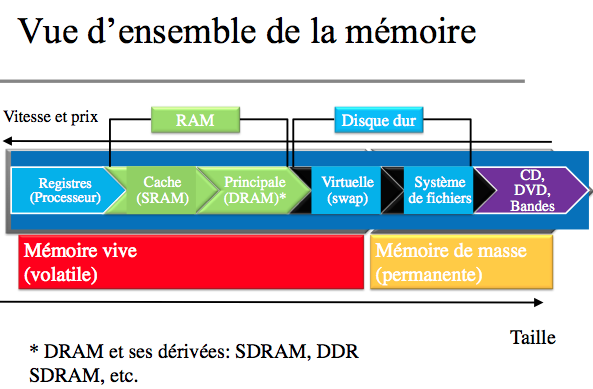
\includegraphics[ scale=0.5]{memo2}
\end{center}

\begin{center}
	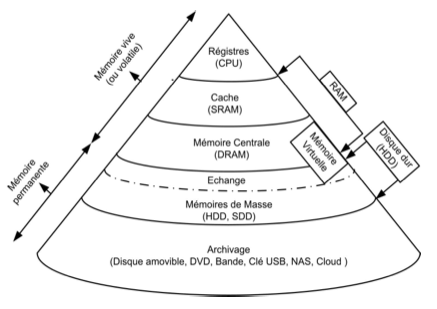
\includegraphics[ scale=0.6]{mem2}
\end{center}
On notera sur la pyramide ci-dessus que plus on descend, plus il y a de place disponible dans la mémoire mais moins les accès y sont rapides et donc moins ces mémoires sont coûteuses.

\section{Première description de la mémoire centrale}

Les mémoires {\bf RAM }, ou Random Access Memory sont qualifiées de  Random par référene à la manière dont on y accède. En effet quelque soit l'emplacement d'un octet (qui peut en effet être aléatoire), son accès se fait de la même manière et prend le même temps. Dans le registre d'instruction mémoire MA on sélectionne une ligne ( CF schéma plus bas) de 8 bits (généralement instructions codées sur 32 ou 64 bits  $\rightarrow$ on prend 4 ou 8  lignes). C'est un mode d'accès fondamentalement différent de l'accès séquentiel.En effet,à part pour la mémoire RAM, les temps d'accès dépendent de la position de l'information..\\
La mémoire centrale se trouve reliée aux autres éléments de l'ordinateur par des liaisons fonctionnant à des vitesses et des largeurs de bus en croissance incessante, la rapidité de ces liaisons étanr un élément influant la performance des systèmes. Mais le débit de la mémoie centrale est loin d'avoir suivi l'évolution des performances des processeurs et il n'est pas en mesure d'alimenter le processeur en donnéees et en instructions à une cadence suffisante pour lui permettre d'atteindre sa pleine performance. C'est pourquoi il y a généralement à proximité du processeur une ou plusieurs mémoires de capacité réduite mais présentant des temps d'accès sérieusement réduits. {\bf Cette réduction est donc obtenue par l'utilisation de mémoire d'un type beaucoup plus rapide et par la proximité de celle-ci ainsi qu'à l'usage exclusif du processeur}. Ce sont les mémoires {\bf caches} introduites dans la partie traitant du processeur, et qui contiennent une copie exacte du contenu d'un très petit nombre de blocs de la mémoire centrale. Ces blocs reprennent les données les plus fréquemment et récemment utilisées en se basant sur le principe de localité mais nous reviendrons plus loin sur le fonctionnement de la mémoire cache. Elles sont toutes deux, ainsi ques les régistres du processeur, des mémoires {\bf volatiles}. C'est-à-dire qu'elles ne peuvent fonctionner que si elles sont sous alimentation en courant électrique. Une fois le courant coupé, le contenu disparaît. C'est pourquoi l'ordinateur nous invite à sauver notre travail avant de s'éteindre. En pratique cette sauvegarde revient à recopier les données en cours d'édition de la mémoire centrale vers {\bf le support de stockage de masse} ( le disque dur généralement).

\section{Mémoires spécialisées, mémoires secondaires et mémoires d'archivage }

\subsection{Mémoires spécialisées}
Diverses mémoires spécialisées sont utilisées pour assurer le fonctionnement de certains organes de l'ordinateur. On citera uniquement les tampons ou {\bf buffers} qui sont des mémoires généralement intercalées entre les périphériques et la mémoire centrale et qui permettent d'accélérer notablement certaines opérations d'entrée-sortie en anticipant sur la fin d'une opération d'écriture sur le périphérique ou en mémorisant des données utilisées répétitivement. C'est le même principe d'optimisation que celui utilisé avec la mémoire cache, où on interpose un élément plus rapide agissant de manière transparente, ici avec les périphériques et avec le processeur pour la cache.

\subsection{Mémoires secondaires ou de masse}
Il s'agit là du {\bf deuxième niveau} de mémoire dont le principal représentant est le {\bf disque dur} sur lequel les données sont écrites sous forme de champ magnétique ou d'aimantation, {\bf non volatiles} cette fois. Ces mémoires secondaires sont localisées en dehors de l'unité centrale,et par opposition avec les mémoires centrales, leur contenu est accessible à tout moment dès lors que ces supports sont reliés à l'ordinateur. A nouveau par opposition avec la mémoire centrale, leurs temps d'accès peut dépendre de l'emplacement auquel on souhaite accéder. Plus précisément ce temps d'accès dépendra de la position courante de la tête de lecture et du temps recquis pour que celle-ci se rende à l'emplacement désiré ( =temps de latence). De plus la taille des cellules transférées ( Cf section transfert de niveaux) vers la mémoire centrale sera beaucoup plus grande, par exemple de 4096 octets ! Cette plus grande taille de blocs d'information à transférer s'explique par la lenteur de l'accès à la mémoire secondaire, d'où l'intérêt de limiter les accès et de ramener des gros blocs mais on en rediscutera plus bas.\\
{Le contenu de la mémoire centrale étant le seul accessible par le processeur ou par les unités périphériques, toute données indispensables à ces derniers et contenue dans le disque dur se devra de transiter vers la mémoire centrale). Donc les mémoires secondaires sont indispensables au fonctionnement de l'ordinateur car elles ont la responsabilité de stocker tous les programmes susceptibles de s'exécuter à un moment ou à un autre ( y compris les plus vitaux tel le système d'exploitation). Avant de se trouver dans la mémoire centrale et donc en cours d'exécution, ces programmes seront obligatoirement stockés sur le ou les disques durs. C'est ce transfert qui se passe quand on double-clique sur une icone de notre écran.\\
Le fait que l'accès à ces mémoires secondaires soit {\bf permanent et direct}, au-delà du rôle de {\bf premier hangar de stockage de l'information}, de leur attribuer un second rôle d'{\bf extension de la mémoire centrale}, en repoussant ainsi les contraintes liées à la taille et au prix de celle-ci. C'est le principe de la {\bf mémoire virtuelle} qui sera approfondi plus loin.

\subsection{Mémoires d'archivage}
Typiquement les supports dits amovibles tels que les clefs USB ou les disques durs externes, on encore comme dans le passé les bandes magnétiques, les cassettes et disquettes,... Beaucoup d'espace mais temps d'accès très long, l'opposé des registres sur la pyramide de la section 3.2.\\



\section{Les transferts de niveau}

\begin{center}
	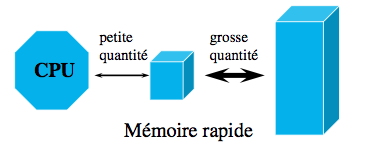
\includegraphics[ scale=0.8]{hierarchie2}
\end{center}

Il existe deux niveaux de mémoire: une rapide transférant à haute fréquence peu de données, l'autre plus lente transférant moins fréquemment beaucoup de données.

Quand PHO va chercher une instruction/opérante, il veut la trouver d'abord dans la mémoire rapide, la chère et petite. S'il ne trouve pas il doit aller chercher dans la grande et plus lente et encore s'il ne trouve pas il va chercher dans le disque dur $\rightarrow$ De plus en plus lent.\\
Mais PHO est malin. Il ne va pas "juste" chercher ce qui manque mais aussi un peu tout ce qu'il y a autour. On dit qu'il ramène des {\bf blocs} ou {\bf pages} dans le cas de la mémoire virtuelle. En effet il y a une forte probabilité que la prochaine chose à prendre ne soit pas loin de la première,tout ceci résume le principe de {\bf localité}, qui est à la fois spatial et temporel.\\
Spatial car on reste dans la même zone mémoire, on ramène des blocs donc il y a une possibilité accrue que les prochaines données dont on aura besoin faisaient parties du bloc et sont donc dans la mémoire rapide. Et temporel car on reste souvent avec les mêmes variables et opérandes dans le temps.\\ Cela permet donc de ne pas devoir retourner dans la mémoire lente de si tôt.\\
Comme le modèle New-Yorkais qui attribue à chaque maison un numéro de rue et un numéro dans cette rue, on peut {\bf décomposer l'addresse} en donnant à chaque partie des fonctions différentes, par exemple 16 bits divisés en 8 bits consacrés à l'adresse des octets et 8 bits pour les blocs. On regroupe donc les octets par bloc et une addresse se compose dès lors du numéro de bloc et de l'adresse de la donnée dans le bloc, ce qui permet de déterminer plus efficacement dans quel bloc une donnée se trouve.

\begin{center}
	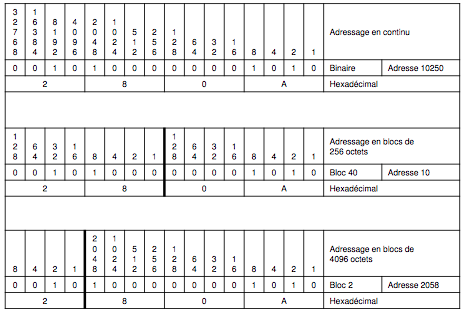
\includegraphics[ scale=0.5]{bloc2}
\end{center}

A Partir du numero du bloc on peut dire si l'adresse concerne une information contenue dans le pemier niveau de mémoire ou dans le deuxième.\\
On dit qu'il y a eu un "raté" si on ne trouve pas ce qu'on cherche dans la mémoire rapide. S'entame alors un long voyage pour aller dans la lente. Il faut minimiser ce taux de raté.

Quand PHO transfère les données en les ramenant, si l'espace est inoccupé dans zone rapide on les met et tout est Ok mais souvent l'espace est occupé,la mémoire rapide est dite saturée, et il est donc nécessaire d'écraser des données pour faire de la place pour accueillir le bloc souhaité par un transfert de niveau Il faut donc effectuer un choix des données à remplacer dans la mémoire rapide.
Alors soit il va éliminer ce qui a été modifé le moins fréquemment possible ou il y a le plus longtemps, ou il va sauvegarder ce qui a été modifié et le mettre dans la mémoire lente.


On notera que ce  principe de fonctionnement est assez semblable entre la mémoire cache et la RAM et dans le cas de la mémoire virtuelle, entre la mémoire centrale et le disque dur.



\section{Fonctionnement de la mémoire centrale}

Nous avons vu plus haut le rôle de la mémoire centrale, qui contient le nécessaire à l'exécution des programmes  par le processeur et le nécessaire pour les échanges avec les unités périphériques. La mémoire centrale porte donc bien son nom, elle est le carrefour central de l'ordinateur, un carrefour encombré car y transitent la plupart des échanges.

On voit sur le schéma ci-dessous l'adressage de la mémoire, dont les accès, rappelons-le, constituent un des feins importants de la performance des ordinateurs.
Les améliorations portent sur la densité des composants afin d'offrir un volume de mémoire plus important, ainsi que sur les mécanismes d'accès, pour réduire le nombre de cycles nécessaires à une opération de lecture ou d'écriture.

Chaque case du schéma est stockée avec un bistable dans le cas de la mémoire Cache et avec un condensateur sinon. {\bf L'adressage} de la cellule est le rôle du registre d'adresses RA (3.1.3) et {\bf les échanges } celui du registre de données RD. En lisant ce qui a dans la ligne on fait passer l'information au registre MD en "tombant".  Toutes les lignes sont donc accessibles à la même vitesse $\rightarrow$ random car ne dépend pas de la position de l'information, l'accès à une cellule n'est pas conditionné par l'accès précédent, comme expliqué dans la première section sur la mémoire centrale.

\begin{center}
	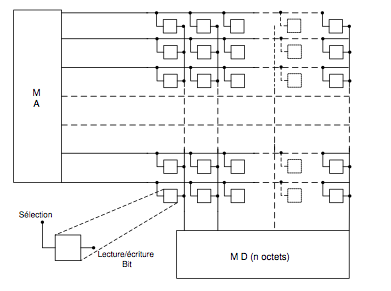
\includegraphics[ scale=0.6]{memoire2}
\end{center}

\section{Mémorisation : DRAM ou SRAM}

La mémoire RAM est elle-même divisée en deux parties :\\ -les {\bf DRAM} ou dynamic RAM, sont les plus utilisées et les moins chères car moins élaborées en électronique et car elles permettent une grande capacité. Mais elles sont en revanche plus lentes (temps d'accès plus lents). Chaque bit est matérialisé principalement par un {\bf condensateur } dont l'état de charge traduit sa valeur binaire.Les condensateurs se déchargent progressivement avec le temps et exigent donc des rafraîchissements du contenu des mémoires très fréquents, d'où leur appellation "dynamic" et leur lenteur car cette opération de rafraîchissement doit être exécutée en priorité par rapport aux autres accès et affecte négativelent kes temps d'accès moyens de la mémoire DRAM. \\
-les {\bf SRAM} ou static RAM, plus rapides et plus onéreuses,fonctionnent avec bistables qui ne nécessitent pas de rafraichissement d'où leur appelation static. {\bf Elles sont utilisées pour les mémoires caches}. \\

Le terme générique DRAM recouvre un sensemble de réalisatoins plus particulières surtout au niveau de l'optimalisation des mécanismes d'accès. Ainsi la {\bf SDRAM} ( synchronous dynamic random access memory) est une mémoire de type DRAM où les accès successifs sont synchronisés avec l'horloge externe du processeur.


Lorsqu'on exécute un programme, une partie est exécutée dans la partie {\bf Cache}, l'autre dans la partie {\bf RAM} (majorité) et le reste dans le {\bf Disque dur} c'est-à-dire en mémoire virtuelle. On fait (quasi) systématiquement un accès disque pour exécuter des programmes.

\section{Le décodeur d'adresses}

\begin{center}
	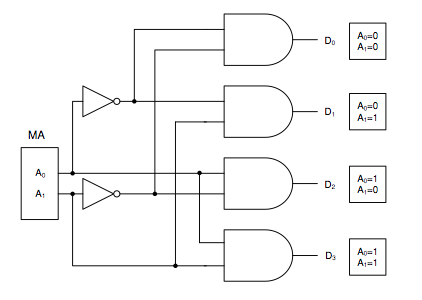
\includegraphics[ scale=0.6]{memoir2}
\end{center}


Sur le schéma ci-dessus est décrit le fonctionnement d'un {\bf décodeur d'adresses}.  Soit un registre mémoire de 2 bits ( MA a 2 bits). Les triangles sont des inverseurs et les autres des "AND" (cf Chap 1). On a donc que si $A_0$ et $A_1$ sont 0, alors $D_0 = 1$ et$D_1 = D_2 = D_3 = 0$ $\rightarrow$ le couple 0;0 donne la ligne 1 et par le même raisonnement le couple 0;1 donne la ligne 2, etc.. Et donc en fonction de $A_O et A_1$ donnés on choisit la bonne ligne par ce principe.\\
NB: Ce décodeur de 2 bits est déjà complexe et la complexité croît exponentiellement avec le nombre de bits !\\

On peut simplifier ceci par des {\bf mémoires bidimensionnelles en 2 phases}, la première affectée à la sélection de la rangée et la deuxième à celle de la colonne. \\ 



\begin{center}
	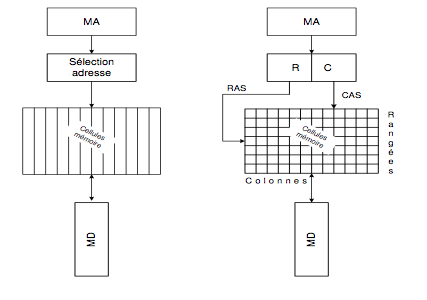
\includegraphics[ scale=0.6]{memoi2}
\end{center}





Il est important de noter qu'il est plus intéressant de saturer la RAM, c'est-à-dire avoir plus de RAM, qu'acheter un processeur qui va 2x plus vite car une fois qu'il n'y a plus de place en RAM il faut aller chercher ailleurs $\rightarrow$ beaucoup plus lent.\\

\section{La mémoire virtuelle}
\subsection{Description}

Avant de décrire le concept de mémoire virtuelle, citons les raisons qui l'ont initiées, soit les raisons qui font que les programmes ne s'accomodent pas bien d'une mémoire centrale :\\
-La taille de la mémoire est insuffisante.\\
-Des parties des programmes sont temporairement superflues.\\
-Il y a une multiplication des programmes présents simultanément.
-Des variations et fractionnement de l'espace mémoire sont disponibles.

Jusqu'à présent on a considéré les octets comme vus dans la mémoire centrale comme une suite linéaire de cellules adjacentes ans un espace à deux dimensions. La réalité est tout autre. Bien sûr, la mémoire centrale ayant les limitations que l'on sait, cet espace idéal ou virtuel ne se traduira pas par un espace contigu de la taille correspondante en mémoire centrale. Un système de gestion de la mémoire, attribuera à chaque programme la partie de mémoire qu'il peut exploiter et s'occupera de la traduction des adresses physiques en adresses réelles( chaque adresse virtuelle est associée à une adresse réelle).Les programmes sont en effet "bluffés", on leur fait croire qu'ils disposent de toute la mémoire souhaitée alors qu'en fait ce qu'ils possèdent est on ne peut plus {\bf virtuel}. On les place en effet au moment de l'exécution à un emplacement quelconque de la mémoire centrale, emplacement choisi et géré par le système d'exploitation. Le système d'adressage interne des programmes n'est en rien modifié, mais il est passé du statut réel à celui de virtuel.Le programme jouera de son espace d'adresses virtuelles comme si celles-ci débutaient à l'adresse zéro de la mémoire centrale et se suivaient en continu. Mais en fait ce programme sera {\bf fragmenté} et dispersé, en partie dans la mémoire centrale et en partie dans la mémoire secondaire. Les fragments s'appelent des "pages".


On voit sur le schéma trois programmes d'application, chacun comprenant un certain nombre de ces pages et se trouvent eclatés dans la mémoire centrale. Cela permet une économie de l'espace avec une plus grande flexibilité lors de l'occupation de celui-ci par des objets de taille très variable.
\begin{center}
	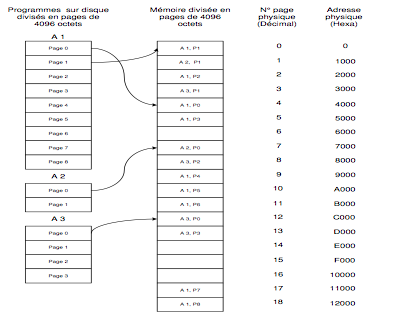
\includegraphics[ scale=0.6]{fragm2}
\end{center}

En fait la gestion de la mémoire centrale est considérablement facilitée en dissociant d'une part l'adressage des cellules tel que le programme le voit( adresses logiques) et d'autre part l'emplacement réel de ces cellules (adresses physiques). La pagination est
un des mécanismes permettant de créer cette dissociation.

Le programme sera donc fragmenté en pages de longueur fixe et sera logiquement organisé comme une succession de ces pages. Ce sont ces mêmes pages qui seront physiquement transférées entre la mémoire centrale et un emplacement de la mémoire {\bf secondaire}.
Cette mémoire secondaire constituera donc une "extension de la mémoire vive". Ce sera donc une partie du disque dur qui ne sera plus accessible pour le stockage permanent des fichiers de l'utilisateur et dont le contenu sera perdu à la fermeture de l'ordinateur.
Le principe d'utiliser le niveau secondaire, donc ici le disque dur, pour étendre la capacité de la mémoire principale, est très utile pour les machines multi-task et pour les serveurs, chaque tâche pouvant utiliser la mémoire principale comme si elle était seule. La mémoire RAM n'étant que de plusieurs Gigas, généralement 2, et les système d'exploitation tels que Windows ou Mac OS en font 4, on comprend bien que l'essentiel de l'espace recquis par le processeur se trouve dans le disque dur.

Si on retourne au schéma de la section 3.2, on voit que la mémoire virtuelle est bien à cheval sur la mémoire centrale et celle d'echange ( disque dur). C'est pour que, comme évoqué plus haut, {\bf les transferts de niveaux demeurent transparents}. Ainsi différents niveaux hiérarchiques sont regroupés sous la même appellation "mémoire virtuelle".

Les avantages : \\
1. Adressage simplifié, relatif au programme.\\
2. Espace mémoire étendu sans augmenter en RAM coûteux.\\
3. Contrôle des adressages dans des espaces réservés au système,pour des raisons de protection, on peut facilement separer les espaces mémoires réservés à différents process(=programmes en train de s'exécuter).

\subsection{La pagination}



Il est intéressant de comprendre les dispositifs qui permettent de traduire en adresses réelles les adresses virtuelles. La page physique sera trouvée idéalement quelque part dans la mémoire centrale. Ceci grâce à une {\bf table des pages} comme sur la figure ci-dessous. Elle est responsable de la mise en correspondance entre l'adresse logique et physique, soit en mémoire centrale  soit en mémoire secondaire. C'est le système d'exploitation qui s'occupe de la création et de la gestion de ces tables des pages. Cette table des pages {\bf est constitutée d'ne liste reprenant pour chacune des pages logiques le numéro de page physique correspondant et d'un indicateur précisant si la page est en mémoire centrale ou secondaire}. 


\begin{center}
	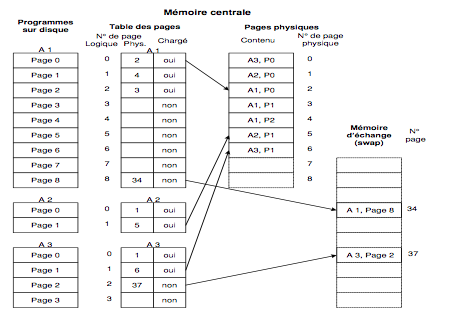
\includegraphics[ scale=0.6]{frag2}
\end{center}

\subsection{Gestion des pages : l'unité de gestion de mémoire et TLB : mémoire associative}

La table des pages associée à chaque programme devient le passage obligé avant d'accéder à la mémoire physique. La juxtaposition du numéro de page physique et de la position relative dans cette page est réalisée par la MMU ( Memory Management Unit) ou unité de gestion de mémoire,qui opère à partir des informations contenues dans la table des pages. En général il y a un MMU par programme. Si l'adresse logique de la page n'est pas dans la table, c'est un raté. Le CPU doit alors s'interrompre et il faut aller chercher la page sur le disque dur pour la charger dans la mémoire principale.
Normalement, la mémoire virtuelle doit être explorée avant la mémoire cache. Cela peut être long et il faut limiter les accès. L'unité de gestion de mémoire se voit donc adjoindre une mémoire de très petite capacité mais ultrarapide et très spécialisée, la  TLB (Translation lookaside buffer), une toute petite cache qui contient les pages les plus récentes et les plus utilisées, dans la discontinuité et le désordre. Il s'agit d'une mémoire associative car les pages ne sont plus dans une séquence logique et c'est une mémoire qui doit fonctionner très rapidement. Comme pour la table des pages, chaque entrée du TLB reprend le numéro de page physique en mémoire centrale, mais avec en plus le numéro de page logique. {\bf La grande différence avec la table des pages vue précédemment est qu'ici l'accès ne se fait pas par l'adresse mais par le  contenu. } Tous les numéros de page logique sont donc comparés une seule fois avec le numéro recherché. C'est ce qui la rend ultrarapide. dans le cas du TLB, au terme de la recheche par le contenu et exhaustive en un coup, si le numéro de page logique a été trouvé, le numéro de la page physique est généré automatiquement par l'unité de gestion de mémoire. Sinon, on passe à la table des pages en mémoire centrale. Voir la section 3.11. 


\begin{center}
	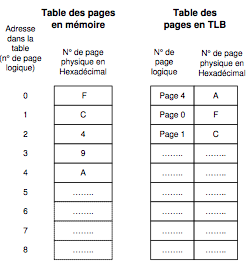
\includegraphics[ scale=0.6]{tlb2}
\end{center}

\section{La mémoire cache}


La technologie des mémoires {\bf Cache} fonctionne sur le principe de biportes et est très chère car plus rapide. Il n'est pas non plus nécessaire de les rafraîchir d'où leur prix élevé. Elles sont à portée immédiate du processeur, reprenant une copie des instructions et des données les plus fréquemment ou récemment utilisées.\\




Sur le schéma ci-dessous on peut observer le fonctionnement de la cache. L'adresse est décomposée en 3 parties : {\bf tag},{\bf ligne} et {\bf adresse de l'octet dans la ligne}.C'est donc à nouveau un mécanisme de localisation basé sur la scission de l'adresse. Le tag est une notion importante, il donne la position relative de chaque bloc, il permet de retrouver la position d'origine de l'ensemble dont est extrait la ligne dans la mémoire centrale. Il est nécessaire de tenir une correspondance parfaite entre la cache et la RAM, c'est-à-dire savoir pour tout item de la cache d'où il vient dans la RAM. C'est ce qu'effectue le tag. Par exemple pour un tag = 9 correspond l'emplacement 9 dans la mémoire centrale. Il suffit de mémoriser dans la {\bf tag table} pour chaque ligne de cache la valeur du tag afin de déterminer à quelle partie d'origine de la mémoire centrale correspond cette donnée.
\begin{center}
	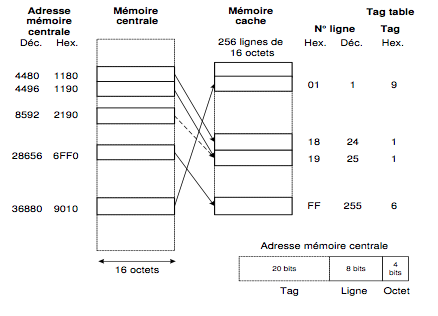
\includegraphics[ scale=0.6]{cache2}
\end{center}


\section{Scénario compet de l'accès à la mémoire}}

L'existence des différents niveaux de mémoire(cache,secondaire,..) et des dispositifs qui leur sont associes (tag table, MMU, TLB,...) rend la gestion de la mémoire très complexe et c'est l'une de taches lesp lus exigeantes de l'OS. Le schéma ci-dessous est {\color{red} important}. Son explication est donnée à la page 128 du livre.

\begin{center}
	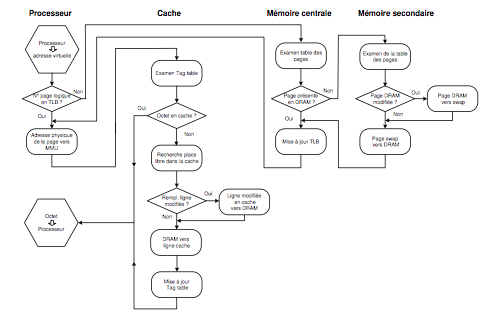
\includegraphics[ scale=0.8]{cach2}
\end{center}


\section{Interconnexions dans l'unité centrale}


Au niveau des interconnexions dans l'unité centrale, les élèments sont reliés par des {\bf bus} qui sont des fils élctriques. ( Cf schéma)\\
Il existe différentes technologies, avant on utilisait plutôt un seul bus , dit passif, qui reliait tous les composants, mais comme cela induit des problèmes de vitesse dûs aux composants lents (les autres plus rapides doivent donc s'ajuster aux plus lents...), il y a actuellement aujourd'hui majoritairement des bus multiples, parallèles ou en série. En série c'est typiquement les cables USB, plus facile car pas besoin de synchronisation comme les parallèles mais par contre à vitesse plus lente. Seulement, les nouveaux bus présentent le désavantage de ne plus etre compatible avec certains périphériques dont la technologie n'a pas évoluée.


\begin{center}
	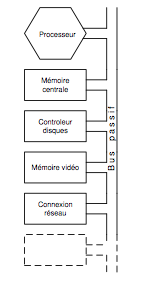
\includegraphics[ scale=0.8]{cac2}
\end{center}

\newpage
\section{Jeu de composants}

L'alternative à la problématique des bus est celle du {\bf chipset} ou "assemblage de composants". Elle consiste à regrouper les composants de l'ordinateur en des ensembles distincts et spécialisés en fonction de leurs besoins en termes de performance et {\bf d'ensuite} créer des points de jonction.
Les composants sont agencés suivant deux types de configuration : rapide dans le NorthBridge et lent dans la partie Sud, qui connecte tous les autres périphériques. La carte mère est le squelette de l'ordinateur, dans laquelle on installe les composants.

\begin{center}
	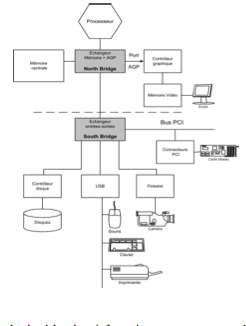
\includegraphics[ scale=0.8]{ca2}
\end{center}

\end{document}